\documentclass[12pt]{article}

\usepackage{times,fullpage,xspace,fancyhdr,url}
\usepackage[pdftex]{graphicx}
\usepackage[pdftex,
            a4paper,
            colorlinks=true,
            urlcolor=black,
            linkcolor=black,
            citecolor=black,
            bookmarksopen=false,
            bookmarksnumbered=true,
            pdfstartview=FitH]{hyperref}

\usepackage{graphicx}
\usepackage{xspace,color}
\pdfcompresslevel=9
\newcommand{\leaguename}{RoboCup Standard Platform League (NAO) }
\hypersetup{
 pdftitle={\leaguename Technical Challenges 2014},
 pdfauthor={Technical Committee},
}
\usepackage[latin1]{inputenc}
\usepackage{amsmath}
\usepackage{times}

% comment 'disable' in to disable all the todo notes :)
\usepackage
[
%disable
]{todonotes}

\sloppy
\newcommand{\ie}{\mbox{i.\,e.}\xspace}
\newcommand{\eg}{\mbox{e.\,g.}\xspace}
\newcommand{\cf}{\mbox{cf.}\xspace}
\newcommand{\comment}[1]{\marginpar{\pdfannot width 4in height .5in depth 8pt {/Subtype /Text /Contents (#1)}}}
\newcommand{\inparagraph}[1]{\paragraph{#1\hspace{-1em} }}


% some colors
\definecolor{orange}{rgb}{1,0.5,0}
\definecolor{red}{rgb}{1,0,0}
\definecolor{green}{rgb}{0,1,0}


\title{\leaguename \\ Technical Challenges}
\author{RoboCup Technical Committee}
\date{(2014 rules, as of \today)}

\setlength{\parindent}{0pt}
\setlength{\parskip}{6pt plus 6pt minus 3 pt}
\setcounter{tocdepth}{1}
\widowpenalty=10000
\clubpenalty=10000

\pagestyle{fancy}
\lhead{}
\chead{}
\rhead{}
\lfoot{}
\cfoot{}
\rfoot{}

\renewcommand{\headrulewidth}{0.4pt}
\renewcommand{\footrulewidth}{0.4pt}

% needed to align an image and text correctly side by side
\newcommand{\imagebox}[1]{\raisebox{2ex}{\raisebox{-\height}{#1}}}



\begin{document}

\maketitle

At RoboCup 2014, the Standard Platform League will hold three different technical challenges, which are described in this document.

The scores earned in each challenge will vary in magnitude.  Hence, they must be scaled before calculating the overall technical challenge rankings.  Teams who do not participate in a challenge will receive 0 points for that challenge.  The team with the highest total score for a challenge will get 25 points for that challenge, while the team with the lowest total score for a challenge will get 5 points for that challenge.  A linear equation will then be fit to these two points, and each other participating team in that challenge will gain points for that challenge based on this equation.

Questions or comments on these rules should be mailed to {\small \url{rc-spl-tc@lists.robocup.org}}.

\vfill

\renewcommand\contentsname{Challenges}
\tableofcontents
\setcounter{tocdepth}{1}

\thispagestyle{fancy}

\clearpage

\cfoot{\thepage}
\setcounter{page}{1}



% % % % % % % % % % % % % % % % % % % % % % % %



\section{Open Challenge}
\newcommand{\openMinNum}{three}

This challenge is designed to encourage creativity within the Standard 
Platform League, allowing teams to demonstrate interesting research in 
the field of autonomous systems. Each team will be given \openMinNum{} 
minutes of time on the RoboCup field to demonstrate their research.

Each team that wishes to compete in this challenge \emph{must} send a 
short, one page document describing their demonstration to the technical 
committee by \textbf{June 21, 2014}.  This document should be written to 
convince the technical committee that the demonstration will be (1) interesting 
to the RoboCup SPL community, (2) feasible to show in \openMinNum{} minutes, and 
(3) adheres to all the guidelines given below. The technical committee will review 
the documents, and notify teams whether their proposed demonstrations are 
acceptable.  Teams who do not submit this description by 
the deadline will not be allowed to compete in this challenge. These 
descriptions will be posted on the website before the competition.

The winner will be decided by a vote among all the SPL teams, although the technical 
committee retains the ability to disqualify any teams that give presentations that do 
not adhere to the following guidelines:

\begin{itemize}
\item 
The demonstration must be strongly related to the scope of the league. 
Irrelevant demonstrations, such as dancing and debugging tool presentations, 
are not allowed.
\item
The demonstration must be done in real time, using at least one active NAO robot.  Conference style talks and/or videos are not allowed.
\item 
Each team may use any number of Aldebaran NAO robots. Teams must arrange
for their own robots.
\item 
Teams have \openMinNum{} minutes to demonstrate their research. At most one 
additional minute may be used for initial setup. Any demonstration deemed
likely to require excessive time will be disallowed by the technical
committee.
\item 
Teams may use extra objects on the field as part of their
demonstration. \emph{Robots other than the NAOs may not be used}.
\item 
The demonstration must \emph{not} mark or damage the field. Any
demonstration deemed likely to mark or damage the field will be
disallowed by the technical committee.
\item
The demonstration may \emph{not} modify the NAO robots.
\item 
The demonstration may use off-board sensors or actuators, as long 
as the NAO is still the focus of the challenge.  This is the only 
challenge in which off-board sensors or actuators are allowed.
\item 
The demonstration may use off-board computing power connected over the
wireless LAN. This is the only challenge in which off-board
computation is allowed.
\item 
The demonstration may use off-board human-computer interfaces. This
is the only challenge in which off-board interfaces, apart from the
Game Controller, are allowed.
\end{itemize}

The winner will be decided by a vote among the SPL teams using a Borda
count (\url{http://en.wikipedia.org/wiki/Borda_count}). Each SPL 
team will vote for their top 10 teams in order (excluding themselves).
Teams are encouraged to evaluate the performance based on the
following criteria: technical strength, novelty, expected impact and
relevance to RoboCup. At a time decided by the designated referee,
within one hour of the last demonstration if not otherwise
specified, the captain of each team will submit his or her team's rankings 
by filling out an online form at \url{http://goo.gl/NdCW4p}.  Any points 
awarded by a team to itself will be disregarded. The points awarded by the 
teams will be summed, and the team with the highest total score shall be the winner.

\newpage



% % % % % % % % % % % % % % % % % % % % % % % %



\section{Any Place Challenge}

Unlike humans, which are able to play soccer (at least at a basic level) independent of most environment features (\ie size and color of the ball, lighting, structure of the ground, size of goals, ect), most soccer robots still rely on very strict specifications of their environment. In recent years, the Standard Platform League addressed this issue by removing artificial field elements such as the borders and additional beacons, as well as by holding technical challenges that require playing under varying lighting conditions (2004) and playing with any ball (2009).

This challenge will be about shooting a (standard) ball into a (standard) goal that is not placed on an SPL field but on the floor of some room or hall at the RoboCup venue. The TC will determine the exact place but keep it secret to all participating teams. The chosen place will be challenging but reasonable, \ie, for instance, the ground will be even, hard, and preferably carpeted. There should not be many orange features or yellow walls in the environment.

At the beginning of the challenge, everybody meets at the SPL area. The TC will fetch an official ball and one official goal. Every participating team will bring one robot. From then on, it will not be allowed to change the software or configuration of any robot. The group walks to the place that has been chosen for the challenge. The goal is placed and starting points for the robot and the ball as well as the field of play will be marked. All markers will be (almost) invisible to the robot. The size and shape of the field of play will be similar to a half of the normal SPL field and denotes the area in which the robot has to perform.

When it is their turn, each team will hand their robot to the TC in the penalized state.  The robot will be placed on the starting mark facing in a set orientation (not necessarily towards the goal).  The robot will be put into playing via a chest button press - from this point the robot has a 3 minute running clock to score as many goals as possible.  The robot may score from any position, including on it's first contact with the ball.

After a goal has been scored, the robot will be penalized via a chest button press and then put into playing via a chest button press once it has been placed back onto its starting position and the ball has been placed on its starting point. If the ball goes out of bounds, the ball will be put back on the starting point but the robot will remain in place and no change of state will occur. If a robot is leaving the field of play, it will be penalized via a chest button press, put back on its starting point, and put into playing via a chest button press once on its starting point (but the ball will remain in place).

TC members will handle all movement of the ball and robot during this challenge.
\newpage



% % % % % % % % % % % % % % % % % % % % % % % %



\section{Sound Recognition Challenge}

WLAN communication is one burden SPL robotic soccer has to cope with. As it is neither reliable under tournament conditions nor human-like in any means (rate of data exchange, communication medium), this challenge is the first step towards getting rid of it. To pave the way for acoustic signals and acoustic communication in future RoboCup tournaments, this year's challenge introduces acoustic senses for the teams' robots. The goal of this challenge is to make our robots hear. To be more precise, this year's goal is to make SPL robots recognize specific acoustic signals for game events like game-start and game-stop.

The challenge consists of two major parts:
\begin{description}
	\item[Recognition of predefined signals:] Robots have to recognize predefined static signals emitted by a global sound system. Similar to the horn-like audible alarms in ice hockey, where halftime starts and ends are signaled using the horn, future RoboCup tournaments could rely on this mechanism to signal GameController or referee messages. The predefined acoustic signals are available at \url{http://www.tzi.de/spl/pub/Website/Downloads/soundfiles14.tar.gz}.
	
	\item[Recognition of individual whistles:] Teams should bring one whistle that has to be recognized by the teams' robots. This part of the challenge brings in a ``real soccer'' aspect to the SPL.
	
\end{description}

\begin{figure}[th!]
\centerline{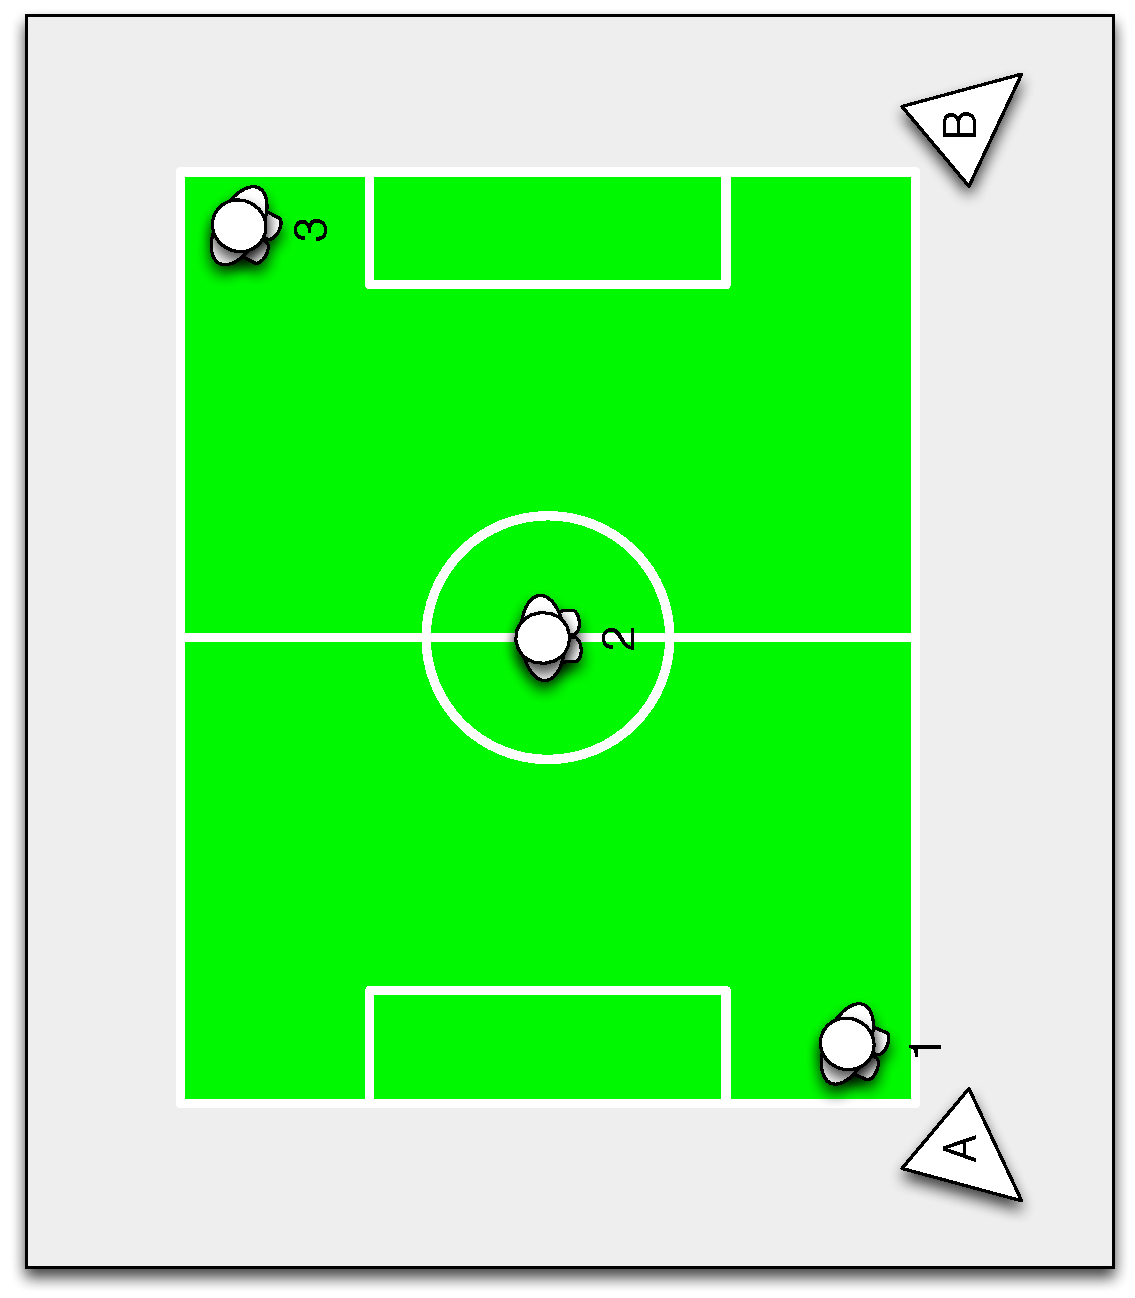
\includegraphics[width=0.6\columnwidth,angle=270]{figures/acuesthesia}}
\caption{Setup for the Sound Recognition Challenge}
\label{fig:recognition_challenge}
\end{figure}

For both parts of the challenge, the field setup is depicted in Figure~\ref{fig:recognition_challenge}. A team has to place one standing robot at each location labeled 1, 2, and 3 in a way such that the robots can not see each other. In addition, robots must look forward and may not move their head. For the first part of the challenge (predefined signals), loudspeakers are mounted at locations A and B. The loudspeakers emit the signals solely and jointly. For the second part of the challenge (whistle), one team member is positioned at a random position on the field to blow the whistle. Provision of additional signals (visual, audible, or WLAN) are prohibited.

Whenever a robot recognizes a given signal, it has to raise at least one arm immediately for about 3 seconds (within one second after the given signal). An arm is considered as \emph{raised}, if the hand is clearly above neck height. In a robot's default pose, both hands are at hip height.
Points are scored by validly recognizing emitted sounds. Falsely detected signals, so raising an arm without given audible alarms, are counted as negative scores and hence are subtracted from the overall score.

The competition procedure will be as follows:

\begin{description}
	\item[Setup:] The team has to place its robots on the field in accordance to Figure~\ref{fig:recognition_challenge}
	\item[Predefined signals recognition:] Each predefined signal is emitted by loudspeaker A. Robots have to signal any detected sound immediately. After a short break, the signal is emitted by loudspeaker B, and after another short break it is emitted by loudspeaker A and B simultaneously. Afterwards, this sequence is repeated once. The overall sequence is the same for each predefined signal. So for two predefined signals it would look like A,B,AB,A,B,AB,A',B',A'B',A',B',A'B' where ' denotes the second predefined signal.\\
	\\For each emitted signal and each robot $1$ point can be achieved. For each false positive $-1$ point will be accounted. For the example sequence, $36$ points can be scored in the best case.
	\item[Whistle recognition:] One team member is placed at a random position on the field simulating a moving main referee. Signaled by the organizers, the teams' whistle is blown once for about one second. After a short break, the team member is relocated to a second random position and repeats the process.\\
	\\ For each emitted whistle blow and each robot, $3x$ points can be scored where $x$ denotes the number of predefined signals from part one of the challenge. For each false positive, $-3x$ point will be accounted. For the example sequence from above, $36$ points can be scored in the best case.
\end{description}

Finally, the overall score is calculated by summing up all points from part one and part two of the challenge.



\end{document}

